\documentclass{standalone}

\usepackage{color}
\usepackage{tikz}
\usetikzlibrary{positioning}


% \definecolor{myred}{RGB}{175,53,71}
% \definecolor{myblue}{RGB}{0,116,188}

\tikzset{
		edgeStyle/.style = {line width = 1.3pt},
		fixed/.style = 		 {anchor=base,fill,circle,inner sep=1pt},
		free/.style =	     {circle,draw},
		node distance=2.3cm
}

\begin{document}
	
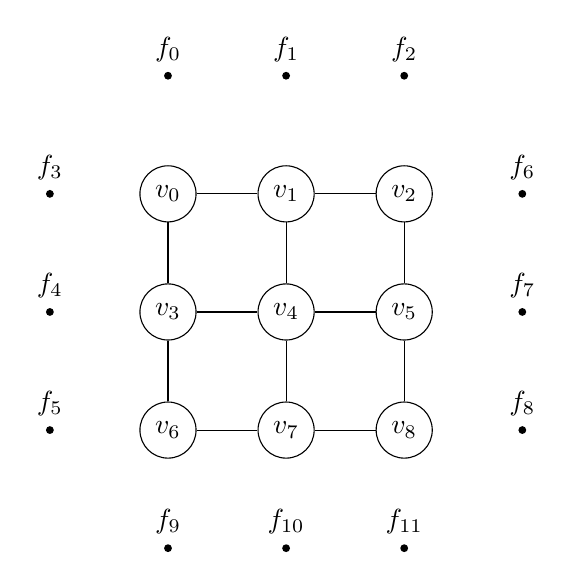
\begin{tikzpicture}
  \newcommand\numFreeRowsCols{3}

  {
    \pgfmathtruncatemacro{\numRowsCols}{\numFreeRowsCols - 1}
    \pgfmathtruncatemacro{\numRowsColsMinusOne}{\numRowsCols - 1}

    % Draw free particles on grid
    \foreach \x in {0,...,\numRowsCols}
      \foreach \y in {0,...,\numRowsCols} 
         {\pgfmathtruncatemacro{\label}{\x - 3 *  \y + 7 - 1}
         \node [free]  (\x\y) at (1.5*\x,1.5*\y) {$v_\label$};} 

    % Draw edges between free particles in grid
    \foreach \x in {0,...,\numRowsCols}
      \foreach \y [count=\yi] in {0,...,\numRowsColsMinusOne}  
        \draw (\x\y)--(\x\yi) (\y\x)--(\yi\x) ;

    % Draw upper row of fixed nodes
    {
      \newcommand\y{\numFreeRowsCols}  
      \foreach \x in {0,...,\numRowsCols}
          \node [fixed] (\x\y) [label=above:{$f_\x$}] at (1.5*\x,1.5*\y) {};
    }

    % Draw lower row of fixed nodes
    {
      \newcommand\y{-1}  
      \foreach \x in {0,...,\numRowsCols}
      {
        \pgfmathtruncatemacro{\label}{\numFreeRowsCols * 3 + \x}
        \node [fixed] (\x\y) [label=above:{$f_{\label}$}] at (1.5*\x,1.5*\y) {}; 
      } 
    }

    % Draw left column of fixed nodes
    {
      \newcommand\x{-1}  
      \foreach \y in {0,...,\numRowsCols}
      {
        \pgfmathtruncatemacro{\label}{(2 * \numFreeRowsCols - 1) - \y}
        \node [fixed] (\x\y) [label=above:{$f_{\label}$}] at (1.5*\x,1.5*\y) {}; 
      } 
    }

    %Draw right column of fixed nodes
    {
      \newcommand\x{\numFreeRowsCols}  
      \foreach \y in {0,...,\numRowsCols}
      {
        \pgfmathtruncatemacro{\label}{(3 * \numFreeRowsCols - 1) - \y}
        \node [fixed] (\x\y) [label=above:{$f_{\label}$}] at (1.5*\x,1.5*\y) {}; 
      } 
    }    

  }

  

\end{tikzpicture}	

\end{document}
